\subsection{1. Unraveling the Mystery: The Purpose of a Single Point Ground Panel!}

\begin{tcolorbox}[colback=gray!10, colframe=black, title=E4E14] What is the purpose of a single point ground panel?
\begin{enumerate}[label=\Alph*.]
    \item Remove AC power in case of a short-circuit
    \item Prevent common-mode transients in multi-wire systems
    \item Eliminate air gaps between protected and non-protected circuits
    \item \textbf{Ensure all lightning protectors activate at the same time}
\end{enumerate} \end{tcolorbox}

\subsubsection{Related Concepts}

A single point ground (SPG) panel is crucial in electrical and communication systems for the effective management of ground potential differences that can occur in various parts of a system. It helps in reducing electromagnetic interference and ensuring that all devices connected to the ground are at the same potential, which is vital for safety and performance. 

The purpose of the single point ground panel is specifically highlighted in option D, which states that its function is to ensure all lightning protectors activate at the same time. This is crucial for protecting sensitive equipment from voltage surges caused by lightning strikes. 

Let's briefly discuss some additional concepts related to this topic:

\begin{itemize}
    \item \textbf{Ground Potential Rise (GPR):} When lightning strikes, the voltage of the ground can temporarily rise, potentially damaging connected equipment if multiple grounding points exist.
    \item \textbf{Electromagnetic Interference (EMI):} Different potential ground points can create loops that pick up interference from external sources, affecting the operation of electronics.
    \item \textbf{Lightning Protection Systems (LPS):} These systems are designed to safely divert the energy from a lightning strike to the ground, and single point grounding is integral to their effectiveness.
\end{itemize}

\subsubsection{Calculation Step}

In scenarios requiring calculation, such as determining the ground potential rise or calculating the required size of grounding elements, we would use Ohm's Law (\(V = IR\)), where \(V\) is the voltage, \(I\) the current, and \(R\) the resistance. 

For example, if the grounding system must handle a lightning strike which induces a current of 30 kA (30,000 A) and the resistance of the ground system is known to be 0.1 ohms, the ground potential rise can be calculated as follows:

\[
V = I \cdot R = 30000 \, \text{A} \cdot 0.1 \, \Omega = 3000 \, \text{V}
\]

This means that during a lightning event, the potential at the grounding system can rise to 3000 volts, emphasizing the importance of a single point ground that effectively manages these potential rises.

\subsubsection{Illustration}

To visualize the concept, a schematic diagram can be created using TikZ. Here is a basic representation of a single point ground panel setup in relation to equipment and lightning protection systems.

\begin{center}
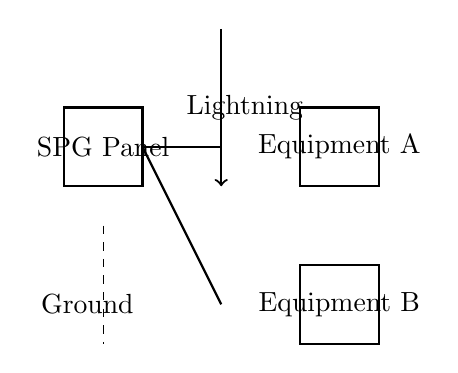
\begin{tikzpicture}
    % Ground panel
    \draw[thick] (0,0) rectangle (1,1);
    \node at (0.5,0.5) {SPG Panel};
    
    % Equipment
    \draw[thick] (3,0) rectangle (4,1);
    \node at (3.5,0.5) {Equipment A};
    
    \draw[thick] (3,-2) rectangle (4,-1);
    \node at (3.5,-1.5) {Equipment B};
    
    % Lightning
    \draw[thick,->] (2,2) -- (2,0);
    \node at (2.3,1) {Lightning};
    
    % Ground connections
    \draw[thick] (1,0.5) -- (2,0.5);
    \draw[thick] (1,0.5) -- (2,-1.5);

    \draw[dashed] (0.5,-0.5) -- (0.5,-2);
    \node at (0.3,-1.5) {Ground};
\end{tikzpicture}
\end{center}
